%\subsubsection{Signal Model and Statistical Procedure} \label{sec:SignalInclusive}
For the integrated or inclusive cross section measurement within the defined region fiducial phase space, a general procedure of differential cross sections measurement as outlined in Section~\ref{sec:StatProcedure} is followed, treating inclusive measurement as a special case where the number of considered bins is  one.
\par 
Table \ref{tab:efficiencySM} shows the reconstruction efficiency ($\epsilon$) for fiducial events, while Table \ref{tab:foutSM} shows the ratio ($f_{nonfid}$)
of events reconstructed from out of fiducial region and the events reconstructed within fiducial volume, per 
final state for different Standard Model signal models. The primary source of the ``nonfiducial signal'' contributions (described with the factor $f_{nonfid}$) 
is the imperfect correspondence of isolation at particle and reconstruction levels, as discussed at the beginning of
Section~\ref{sec:AnalysisStrategy}. 
%The reconstruction efficiency and out of acceptance ratios without including isolation in the fiducial phase space definition
%are shown in Tables~\ref{tab:efficiencySMnoGenIso} and~\ref{tab:foutSMnoGenIso}. 
In a similar way, fraction of the signal events in mass range 105.0--140.0 $\GeV$  where minimum one lepton selected does not originate from the Higgs boson decay are shown in Table~\ref{tab:wrongracSM}.

\begin{table}[!h!tb]
\begin{center}
\small
\caption{
Reconstruction efficiency ($\epsilon$) for fiducial events per final state for different Standard Model signal models at $\sqrt{s} =  13$~TeV with 2018 MC samples.
\label{tab:efficiencySM}
}
\begin{tabular}{|l|c|c|c|c|} \hline
Sample & $4e$ & $4\mu$ & $2e2\mu$ & $4\ell$ \\ \hline
gg$\rightarrow$H ({\sc powheg})  & 0.404 $\pm$ 0.002 & 0.799 $\pm$ 0.002 & 0.572 $\pm$ 0.002 & 0.593 $\pm$ 0.001 \\
VBF ({\sc powheg})  & 0.431 $\pm$ 0.003 & 0.805 $\pm$ 0.002 & 0.586 $\pm$ 0.002 & 0.608 $\pm$ 0.002 \\
WH ({\sc powheg+minlo}) & 0.415 $\pm$ 0.004 & 0.780 $\pm$ 0.003 & 0.580 $\pm$ 0.003 & 0.593 $\pm$ 0.002 \\
ZH ({\sc powheg+minlo})  & 0.428 $\pm$ 0.006 & 0.780 $\pm$ 0.005 & 0.581 $\pm$ 0.005 & 0.597 $\pm$ 0.003 \\
ttH ({\sc powheg}) & 0.429 $\pm$ 0.006 & 0.745 $\pm$ 0.005 & 0.573 $\pm$ 0.005 & 0.585 $\pm$ 0.003 \\
%ggH(NNLOPS) & 0.425 $\pm$ 0.002 & 0.776 $\pm$ 0.002 & 0.578 $\pm$ 0.001 & 0.595 $\pm$ 0.001 \\
\hline
\end{tabular}
\normalsize
\end{center}
\end{table}

\begin{table}[!h!tb]
\begin{center}
\small
\caption{
Ratio of events reconstructed from out of fiducial volume and the events reconstructed within the fiducial region ($f_{nonfid}$) per
 final state in different Standard Model signal models at $\sqrt{s} =  13$~TeV with 2018 MC samples.
\label{tab:foutSM}
}
\begin{tabular}{|l|c|c|c|c|} \hline
Sample & $4e$ & $4\mu$ & $2e2\mu$ & $4\ell$ \\ \hline
gg$\rightarrow$H ({\sc powheg})  & 0.060 $\pm$ 0.002 & 0.046 $\pm$ 0.001 & 0.060 $\pm$ 0.001 & 0.055 $\pm$ 0.001 \\
VBF ({\sc powheg})  & 0.050 $\pm$ 0.002 & 0.037 $\pm$ 0.001 & 0.046 $\pm$ 0.001 & 0.043 $\pm$ 0.001 \\
WH ({\sc powheg+minlo}) & 0.098 $\pm$ 0.004 & 0.058 $\pm$ 0.002 & 0.080 $\pm$ 0.002 & 0.075 $\pm$ 0.001 \\
ZH ({\sc powheg+minlo})  & 0.105 $\pm$ 0.007 & 0.071 $\pm$ 0.004 & 0.091 $\pm$ 0.004 & 0.087 $\pm$ 0.002 \\
ttH ({\sc powheg}) & 0.278 $\pm$ 0.012 & 0.127 $\pm$ 0.005 & 0.193 $\pm$ 0.006 & 0.185 $\pm$ 0.004 \\
%ggH(NNLOPS) & 0.051 $\pm$ 0.001 & 0.046 $\pm$ 0.001 & 0.051 $\pm$ 0.001 & 0.049 $\pm$ 0.001 \\
\hline
\end{tabular}
\normalsize
\end{center}
\end{table}


\begin{table}[!h!tb]
\begin{center}
\small
\caption{
	Signal event fraction in the mass range 105.0--140.0 $\GeV$ where minimum one lepton selected is originating from Higgs decay at $\sqrt{s} =  13$~TeV with 2018 MC samples.
\label{tab:wrongracSM}
}
\begin{tabular}{|l|c|c|c|c|} \hline
Sample & $4e$ & $4\mu$ & $2e2\mu$ & $4\ell$ \\ \hline
gg$\rightarrow$H ({\sc powheg})  & 0.002 & 0.002 & 0.002 & 0.002 \\
VBF ({\sc powheg})  & 0.002 & 0.003 & 0.003 & 0.003 \\
WH ({\sc powheg+minlo}) & 0.036 & 0.031 & 0.042 & 0.037 \\
ZH ({\sc powheg+minlo})  & 0.199 & 0.207 & 0.212 & 0.208 \\
ttH ({\sc powheg}) & 0.175 & 0.156 & 0.164 & 0.163 \\
%ggH(NNLOPS) & 0.003 & 0.003 & 0.004 & 0.003 \\
\hline
\end{tabular}
\normalsize
\end{center}
\end{table}
%%%%%%%%%%%%%%%%%
\begin{figure}[!htbp]
\begin{minipage}{0.5\linewidth}
\centerline{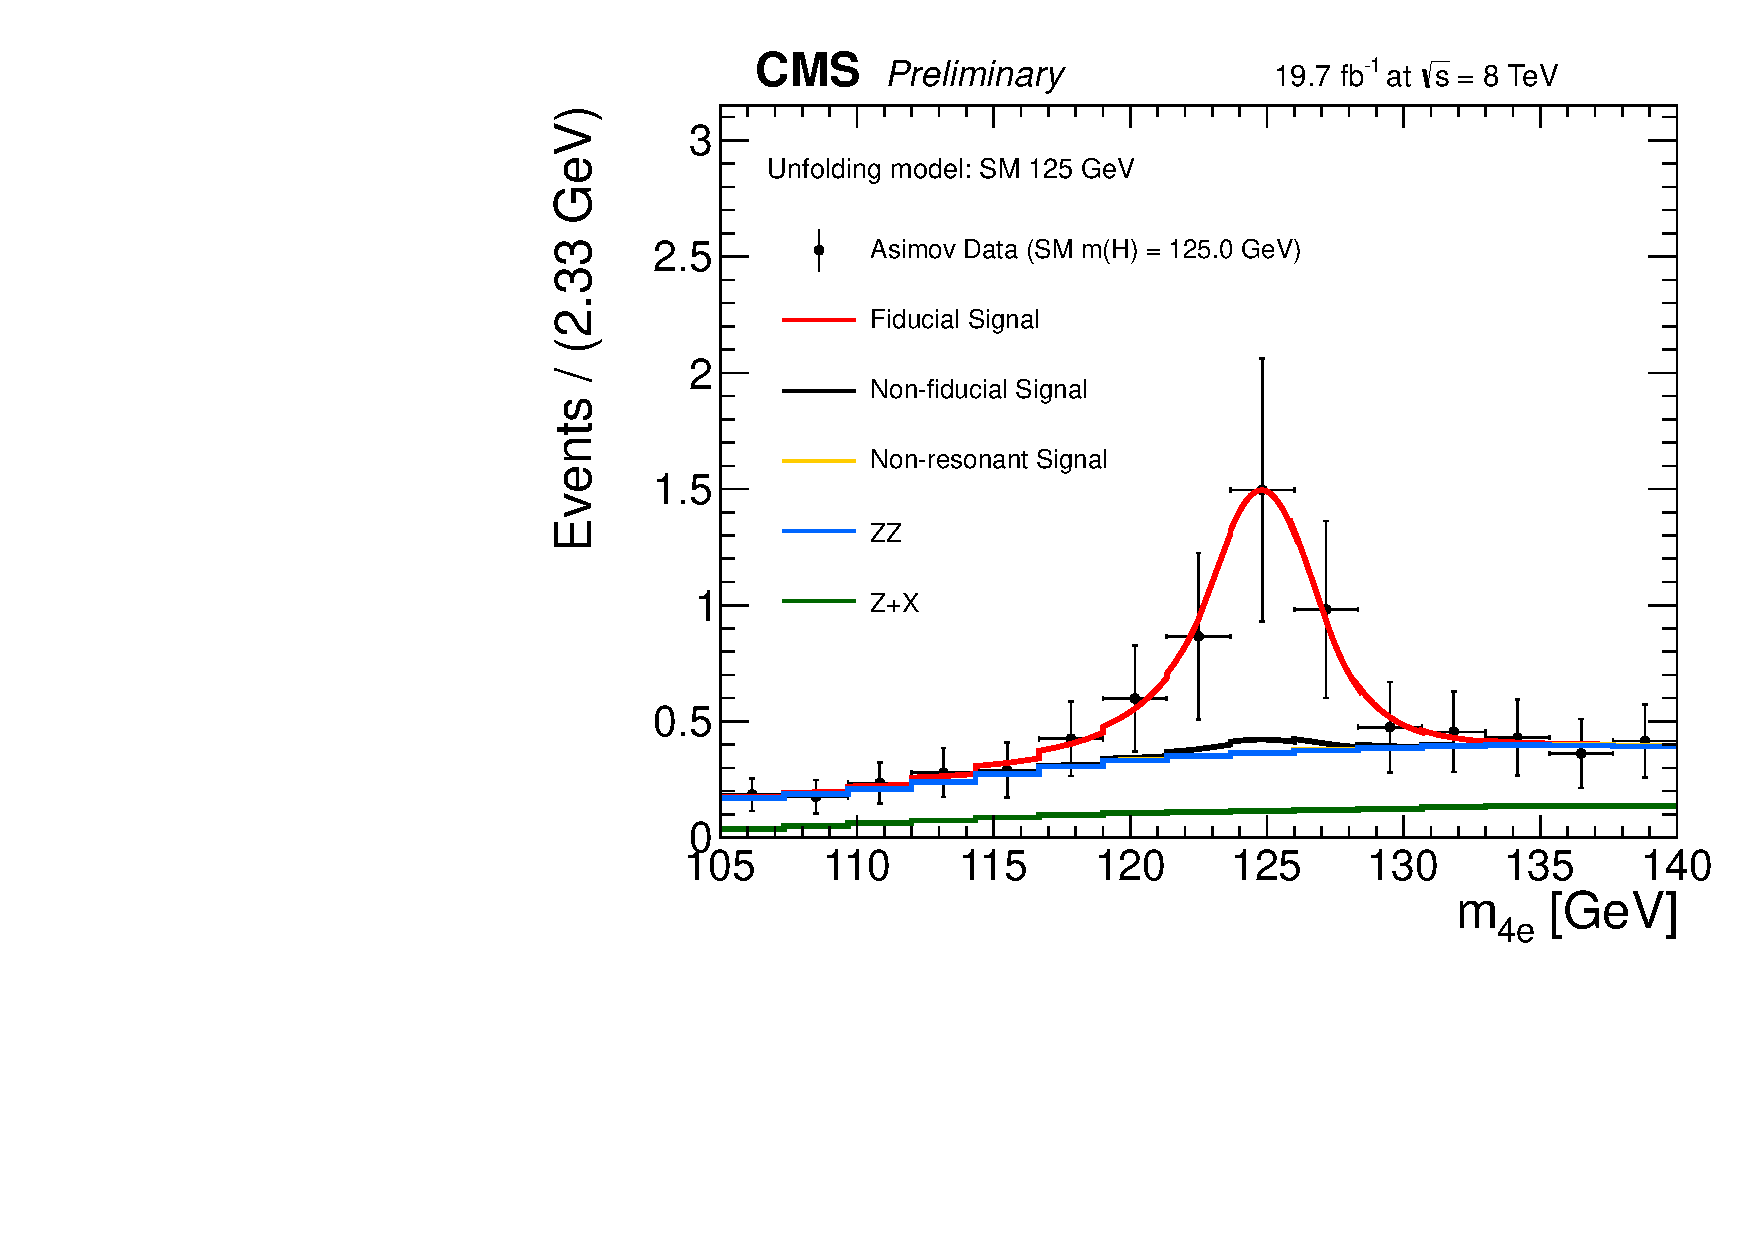
\includegraphics [width=\linewidth] {Plots/asimovdata_SM_125_v2_unfoldwith_SM_125_v2_mass4l_4e_recobin0.pdf}}
\end{minipage}
\begin{minipage}{0.5\linewidth}
\centerline{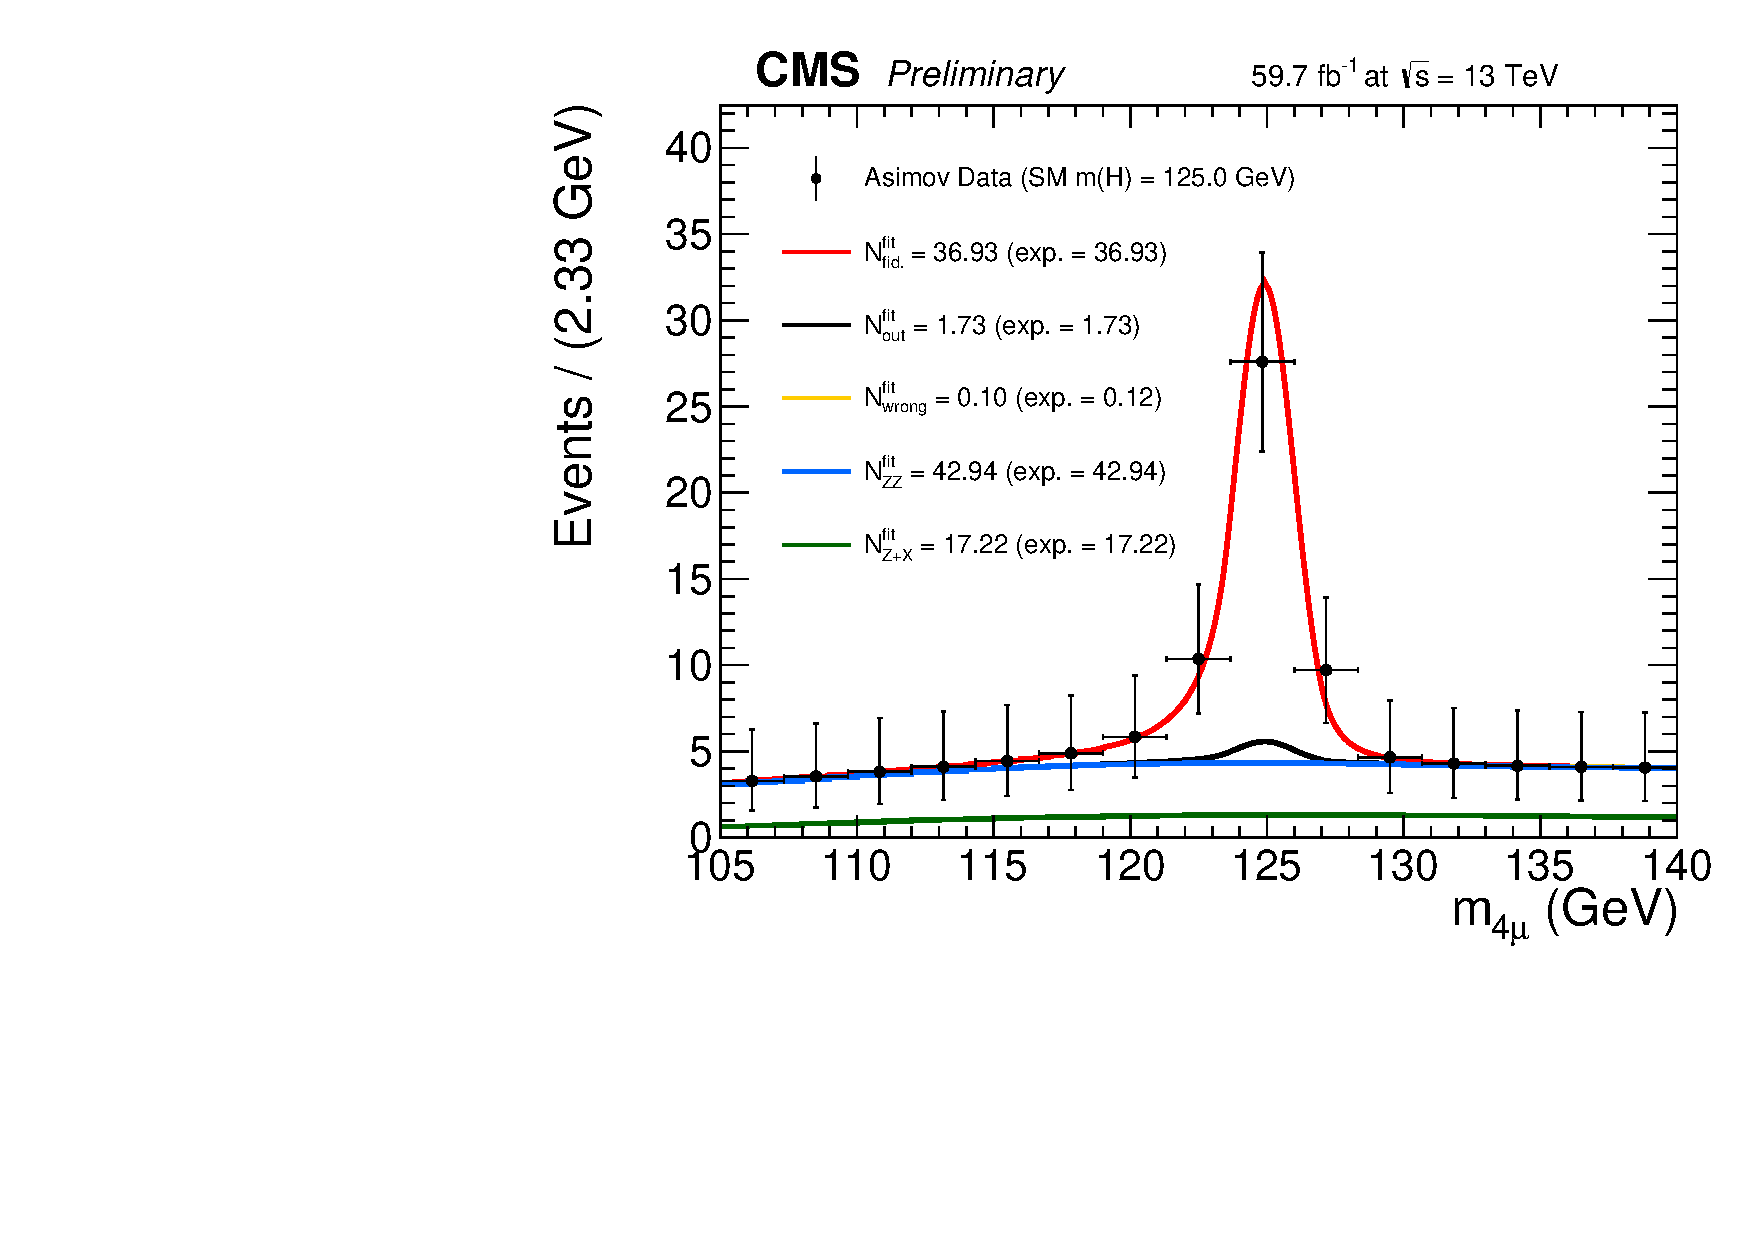
\includegraphics [width=\linewidth] {Plots/asimovdata_SM_125_v2_unfoldwith_SM_125_v2_mass4l_4mu_recobin0.pdf}}
\end{minipage}
\begin{minipage}{0.5\linewidth}
\centerline{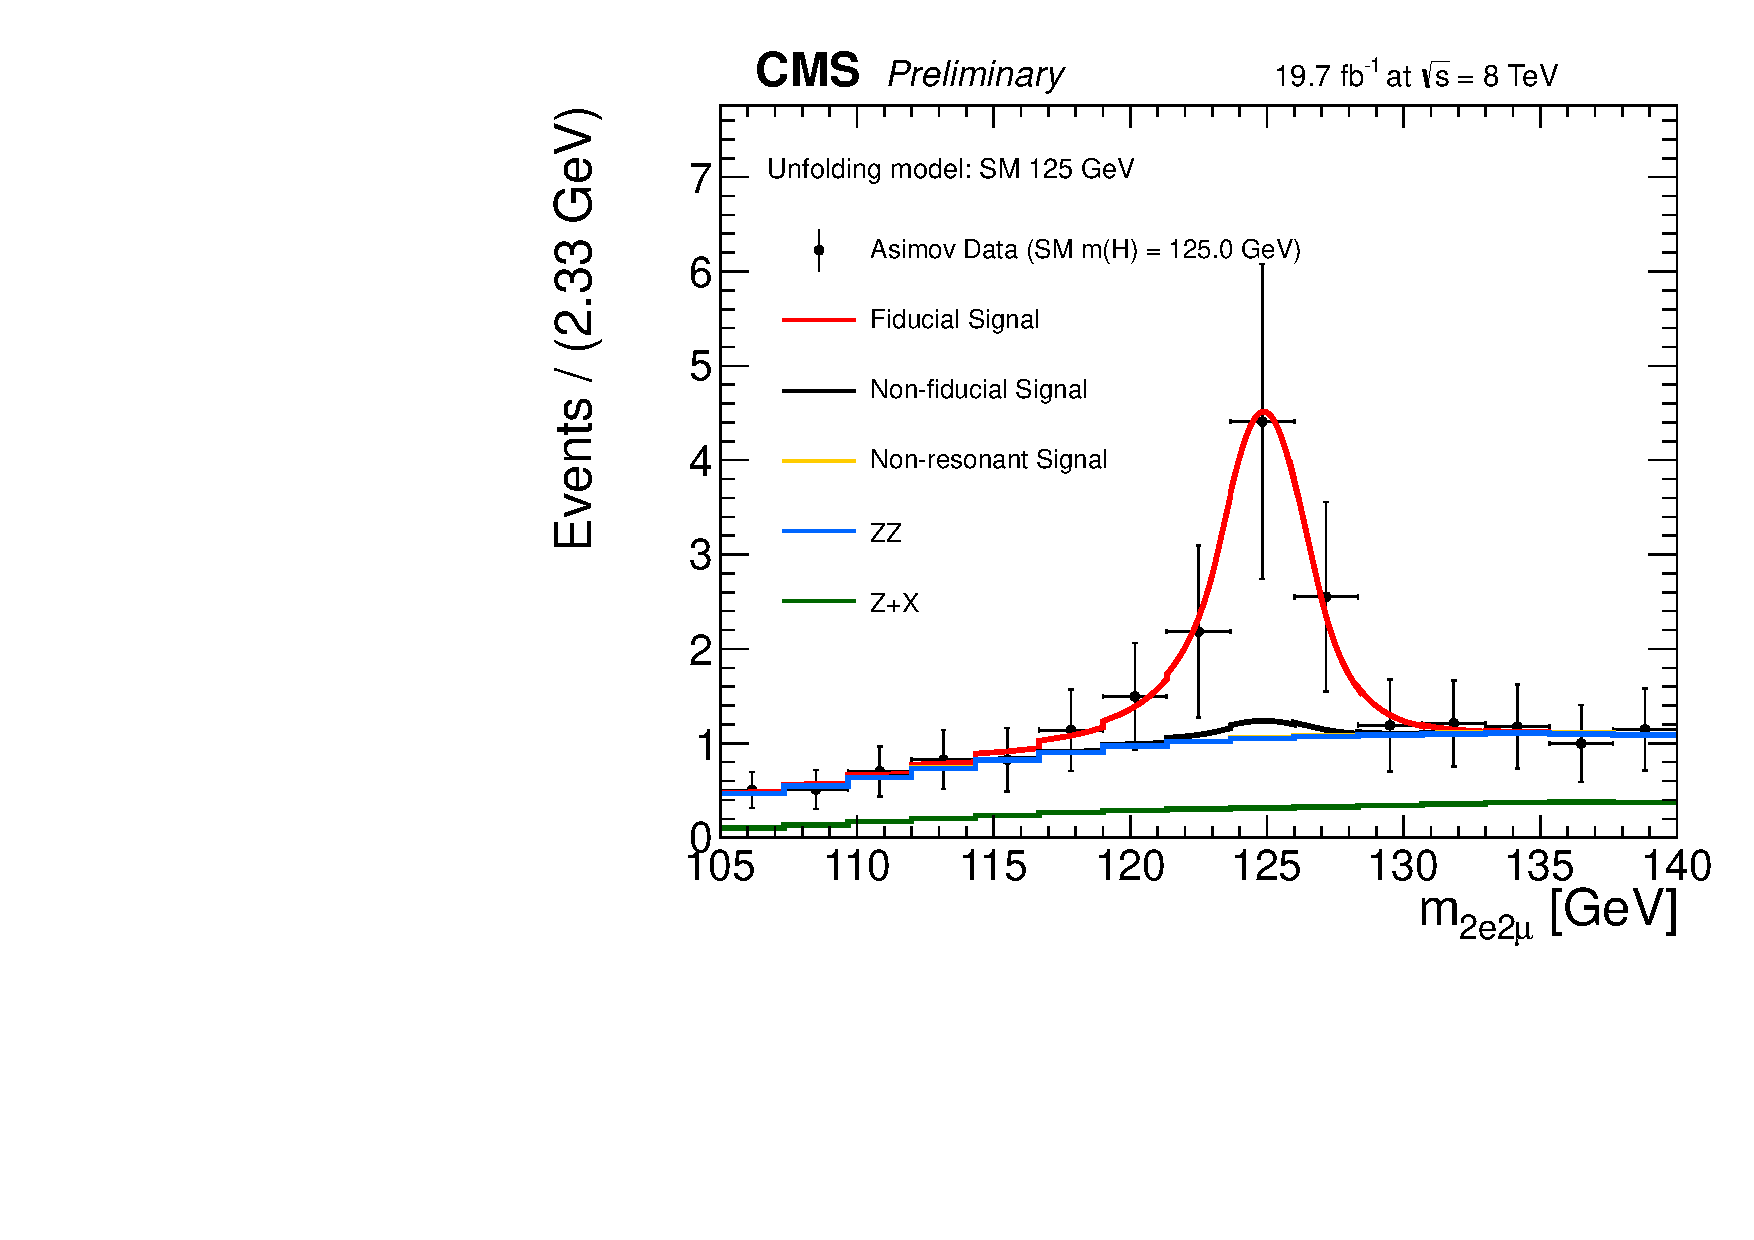
\includegraphics [width=\linewidth] {Plots/asimovdata_SM_125_v2_unfoldwith_SM_125_v2_mass4l_2e2mu_recobin0.pdf}}
\end{minipage}
\begin{minipage}{0.5\linewidth}
\centerline{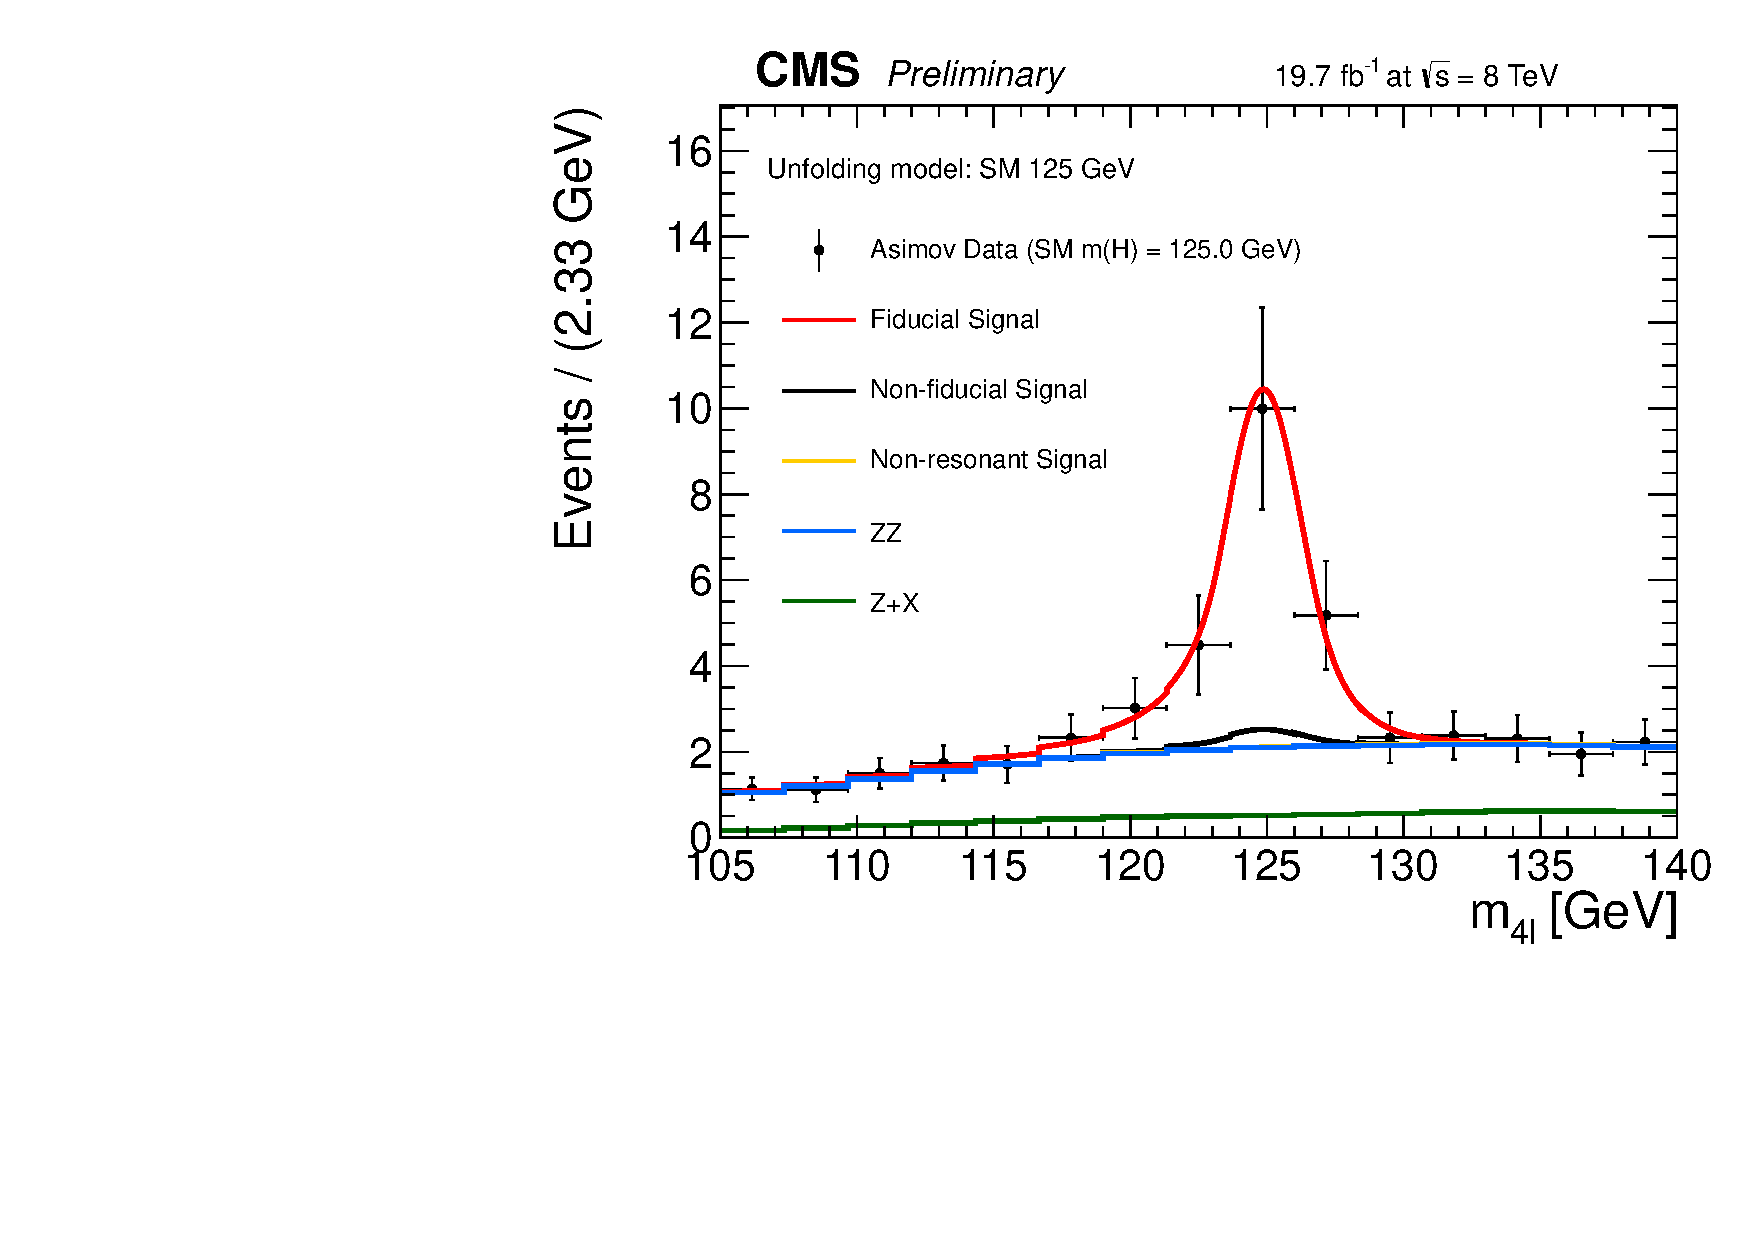
\includegraphics [width=\linewidth] {Plots/asimovdata_SM_125_v2_unfoldwith_SM_125_v2_mass4l_4l_recobin0.pdf}}
\end{minipage}
	\caption{Inclusive four lepton mass distributions for an Asimov Dataset generated using SM cross section values and SM efficiencies where the gg$\rightarrow$H prediction is from {\sc powheg+JHUgen} and resulting fitted values of the signal and background pdfs in different final states at $\sqrt{s} =  13$~TeV with 2018 data.}
  \label{fig:sigfits-asimov-SM-inclusive}
\end{figure}
